\documentclass{article}
\usepackage[margin=1in]{geometry}
\usepackage{problemset}
\showsolntrue

% Custom commands
\newcommand{\R}{\mathbb{R}}
\newcommand{\X}{\mathcal{X}}
\newcommand{\Y}{\mathcal{Y}}
\newcommand{\E}{\mathbb{E}}
\newcommand{\V}{\text{Var}}
\renewcommand{\P}{\mathbb{P}}
\newcommand{\x}{\mathbf{x}}
\newcommand{\w}{\mathbf{w}}

\begin{document}

\pstitle{%
    DSC 180A MA 2%
}{
    Issac Roy%
}[due Monday, October 26 at 11:59PM]

\begin{probset}
% --- Problem 1 ---
\begin{prob}
    What is one thing Dr. Smarr said in the video that you disagree with, or that you think he should have said differently? Use one sentence to identify your concern, and one sentence to offer an alternative that satisfies your concern. Try to constrain your answer to the format of the video (i.e., instead of “he should have talked about this longer” try to offer a rephrasing or alternative topic that would take the same time).

    \begin{soln}
        While he had many great points on how to effectively communicate, I think one section that he skipped out on how to effectively capture someone's attention in the first place, because in my experience, the hardest part is always getting someone to care. 
        
        A lot of the things that he discussed were under the assumption that the other party is willing enough to participate in discussion and he touched a little bit on how to capture attention - such as using audience-based language and stripping away distractions - but he never explicitly identified that getting people to care in the first place is always the hardest step.

        For example, he could gave an example 30-second hook from his own work showing why the audience should care, then used the same time for his tips on audience language.

        P.S. I apologize for more than 2 sentences, I had a lot to say.
    \end{soln}
\end{prob}

% --- Problem 2 ---
\begin{prob}
    Offer critical, constructive feedback about the following sentence. Point out one thing that you feel weakens the sentence, why you feel that way, and provide an alternative:

    Machine learning models are really really good for recognizing the difference between pictures of cats and dogs because they can be deep and because people have spent a lot of time.

    \begin{soln}
        A minor nit is using the word really twice, but perhaps it's for the goal of emphasis. Though other synonyms might be more apt if the aim is to emphasize. ML model is also a vague term since not all ML models are good for this task. The last part is what feels the most wrong "they can be deep and because people have spent a lot of time."

        It never defines what deep means by itself, which is excusable depending on the context, but also fails to tie it to why ML models are really good. Why does depth matter? Additionally, people have spent a lot of time doing what? Labelling the images? The two because clauses also don't match each other, and neither is specific enough to actually explain anything.

        Based on the last phrase, it's difficult to understand what the goal of the sentence is, but I'll provide my alternative on the assumption that it aims to convey why ML models are good.

        Alternative: Some machine learning models such as neural networks are incredibly good at recognizing the difference between pictures of cats and dogs because they are able to leverage latent features such as the shape of the animals' eyes for prediction.
    \end{soln}
\end{prob}

\newpage

% --- Problem 3 ---
\begin{prob}
    You have done a wonderful capstone project. You want to present your work to a company you're hoping hires you, and to your family to show them what you've been doing. Describe two things you would change between these two presentations about the same work you did.

    \begin{soln}
        For the company, I'm assuming that I will be presenting to someone more technical. 

        In this case, they would likely have much more background knowledge than my family members so I could keep my introduction and context shorter and dive into the meat of my project much faster. With my family, I'd either have to keep it at a much higher level or keep providing surrounding context as I go.

        In addition to speed / context, my goals are also different in these cases. With the company, I would present alternatives that I tried and provide the specific technical challenges that I faced and how I cleverly approached them, while with my family, I would likely skip over alternatives and challenges unless they were easy to explain. So overall, context and content highly depends on the audience.
    \end{soln}
\end{prob}

% --- Problem 4 ---
\begin{prob}
    An additional challenge for data visualization is just making sure you didn't leave off important details, and that your data are easy to see. Identify three things you could add or change to improve the following graph's communication efficacy or clarity.

    \begin{center}
        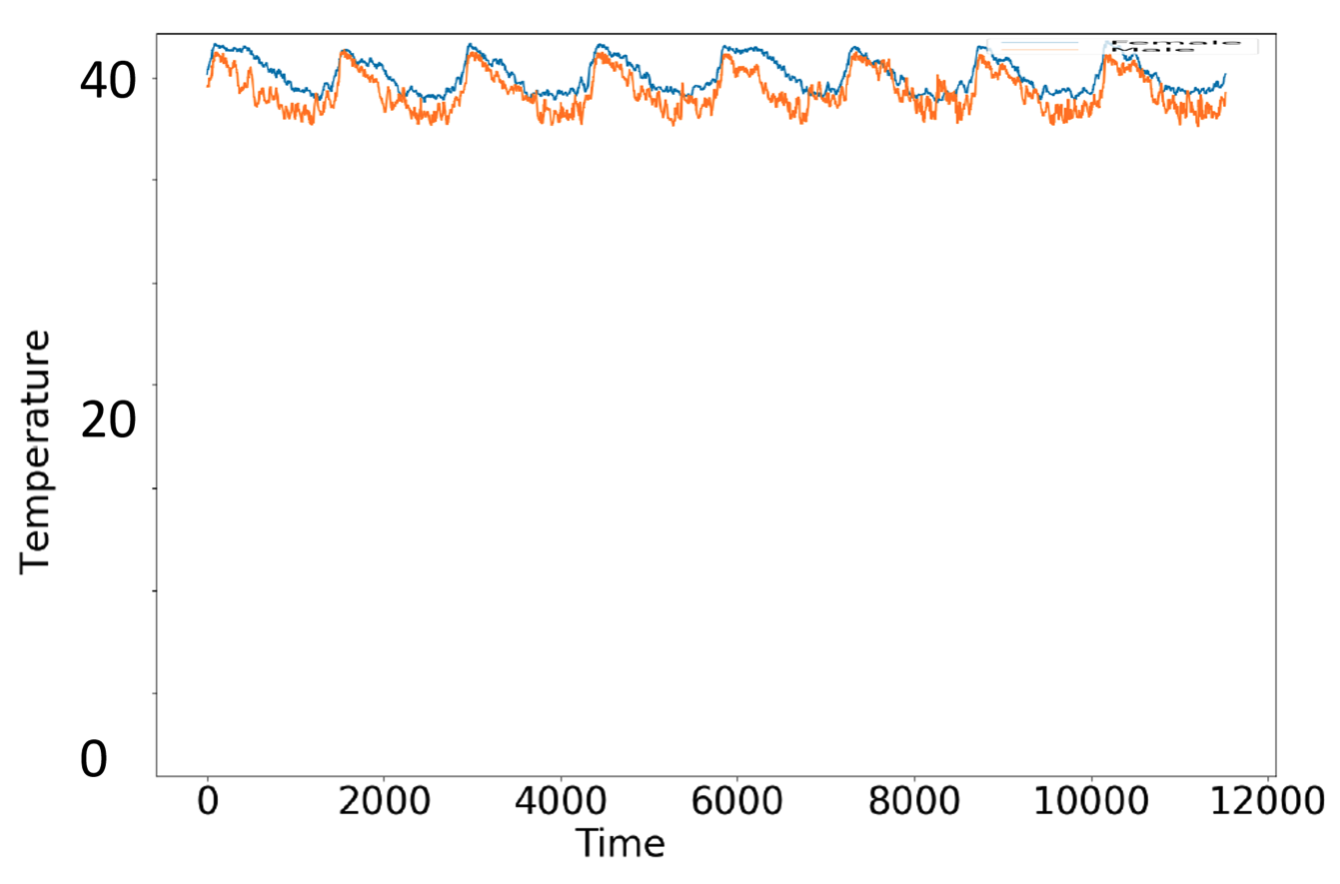
\includegraphics[scale=0.5]{m2-plot.png}
    \end{center}

    \begin{soln}
        There's no title to specify the focus or context. There's no source to specify where the data comes from. Neither axis has units. The legend exists, but is too small to be useful. There's wayyy too much white space. Nit: the x-axis label isn't centered.
    \end{soln}
\end{prob}
\end{probset}
\end{document}